\newcommand{\drawArc}[4]{%Angle1,Angle2,Radius1,Radius2
	\draw[fill=black, line width=0mm]
	(#2:#3) arc
	(#2:#1:#3) --
	(#1:#4) arc
	(#1:#2:#4) --
	cycle;
}

\newcommand{\rotaryEncoderLines}[5]{%Angle1, Angle2, DegreeStep, Radius1, Radius2
	\pgfmathsetmacro{\angleSecond}{#1+#3*2};
	\foreach \a in {#1,\angleSecond,...,#2}
	{
		\drawArc{\a}{\a+#3}{#4}{#5};
	}
}

\newcommand{\drawSimpleRect}[2]{%sizeB sizeB
	\draw[line width=0.1mm] (#1,#2) -- (-#1,#2);
	\draw[line width=0.1mm] (-#1,#2) -- (-#1,-#2);
	\draw[line width=0.1mm] (-#1,-#2) -- (#1,-#2);
	\draw[line width=0.1mm] (#1,-#2) -- (#1,#2);
}

\newcommand{\rotaryEncoder}[4]{%OuterRadius, LineWidth, DetectorAngle, DetectorPulses
	\pgfmathsetmacro{\stepDegree}{2*#3/#4};
	\rotaryEncoderLines{0}{360}{\stepDegree}{#1-#2}{#1};
	\drawArc{\stepDegree}{2*\stepDegree}{#1-#2}{#1};
	\foreach \a in {0,120,240} {
		\draw (\a+90:25mm) circle (3mm);
		\draw (\a+90:25mm) circle (1.5mm);
	}
	\begin{scope}[shift={(0,-31mm)}]
		\drawSimpleRect{9mm}{16mm}
	\end{scope}
	\drawSimpleRect{5mm}{5mm}

	\pgfmathsetmacro{\pulses}{360/\stepDegree};
	\node[draw,rotate=0] (t) at (90:38mm) {Step-$\angle$: \stepDegree$^\circ$};
	\node[draw,rotate=30] (t) at (135:30mm) {Detector-$\Delta$-$\angle$: #3$^\circ$};
	\node[draw,rotate=-30] (t) at (45:30mm) {Detector-$\Delta$-$\sqcap$: #4};
	\node[draw,rotate=0] (t) at (90:15mm) {$\sqcap$: \pulses};
}

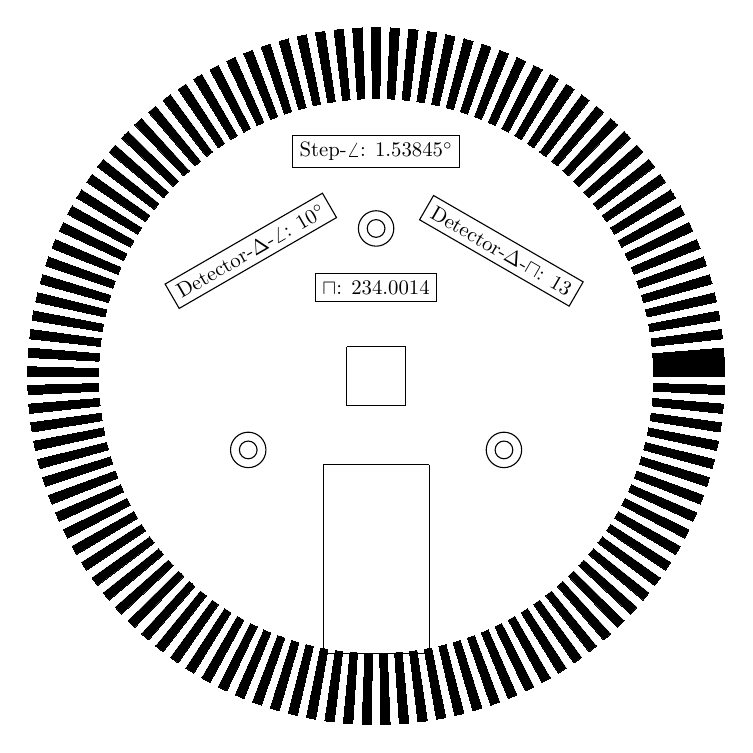
\begin{tikzpicture}[scale=0.75, transform shape]
\rotaryEncoder{59mm}{12mm}{10}{13}
\end{tikzpicture}

